%\documentclass[12pt,a4paper]{article} % POUR TEST
%\usepackage[french]{babel} % POUR TEST
%\usepackage[latin1]{inputenc} % POUR TEST
%\usepackage[T1]{fontenc} % POUR TEST
%\usepackage[UTF8]{inputenc} % POUR TEST
%\usepackage{vmargin} % POUR TEST
%\usepackage{pdfpages} % POUR TEST
%\usepackage{slantsc} % POUR TEST
%\setmarginsrb{2.5cm}{1.5cm}{2.5cm}{2cm}{0cm}{0cm}{0cm}{0cm} % POUR TEST
%
%\begin{document} % POUR TEST

\pagestyle{empty}
{\sffamily
\noindent{Universit\'{e} de Lille \hfill Facult\'{e} de Pharmacie de Lille \\ Ann\'{e}e Universitaire 2023/2024}

\vspace{20mm}
\begin{center}
\textbf{THESE \\
POUR LE DIPLOME D'ETAT \\
DE DOCTEUR EN PHARMACIE}
\end{center}
\vspace{10mm}
\noindent{\textbf{\hspace*{13mm}Soutenue publiquement le 9 novembre 2023 \\
\hspace*{11mm}Par M. RIHANI Emir Ka\"{i}s}}
\vspace{22mm}
\begin{center}
\rule{65mm}{0.8pt} \\
\vspace{4mm}
\textbf{APPLICATION DE MODELES D'APPRENTISSAGE MACHINE \\~\\ A LA CLASSIFICATION DES MACROMYCETES} \\
\vspace{2mm}
\rule{65mm}{0.8pt}
\end{center}
\vspace{32mm}
\noindent{\textbf{\underline{\smash{Membres du jury}} :} \\
~\\
\textbf{Pr\'{e}sident :} \\ 
Pr LEMDANI Mohamed, PU en Biomath\'{e}matiques, Facult\'{e} de Pharmacie de Lille \\
~\\
\textbf{Directeur, conseiller de th\`{e}se :} \\
Dr HAMONIER Julien, MCU en Biomath\'{e}matiques, Facult\'{e} de Pharmacie de Lille \\
~\\
\textbf{Assesseur :} \\
Dr WELTI St\'{e}phane, MCU en Sciences V\'{e}g\'{e}tales et Fongiques, Facult\'{e} de Pharmacie de Lille \\
~\\
\textbf{Membre ext\'{e}rieur :} \\
Dr MOUSSET Caroline, Pharmacien-Ing\'{e}nieur, Responsable AQ Clients, Delpharm Lille
}

\cleardoublepage
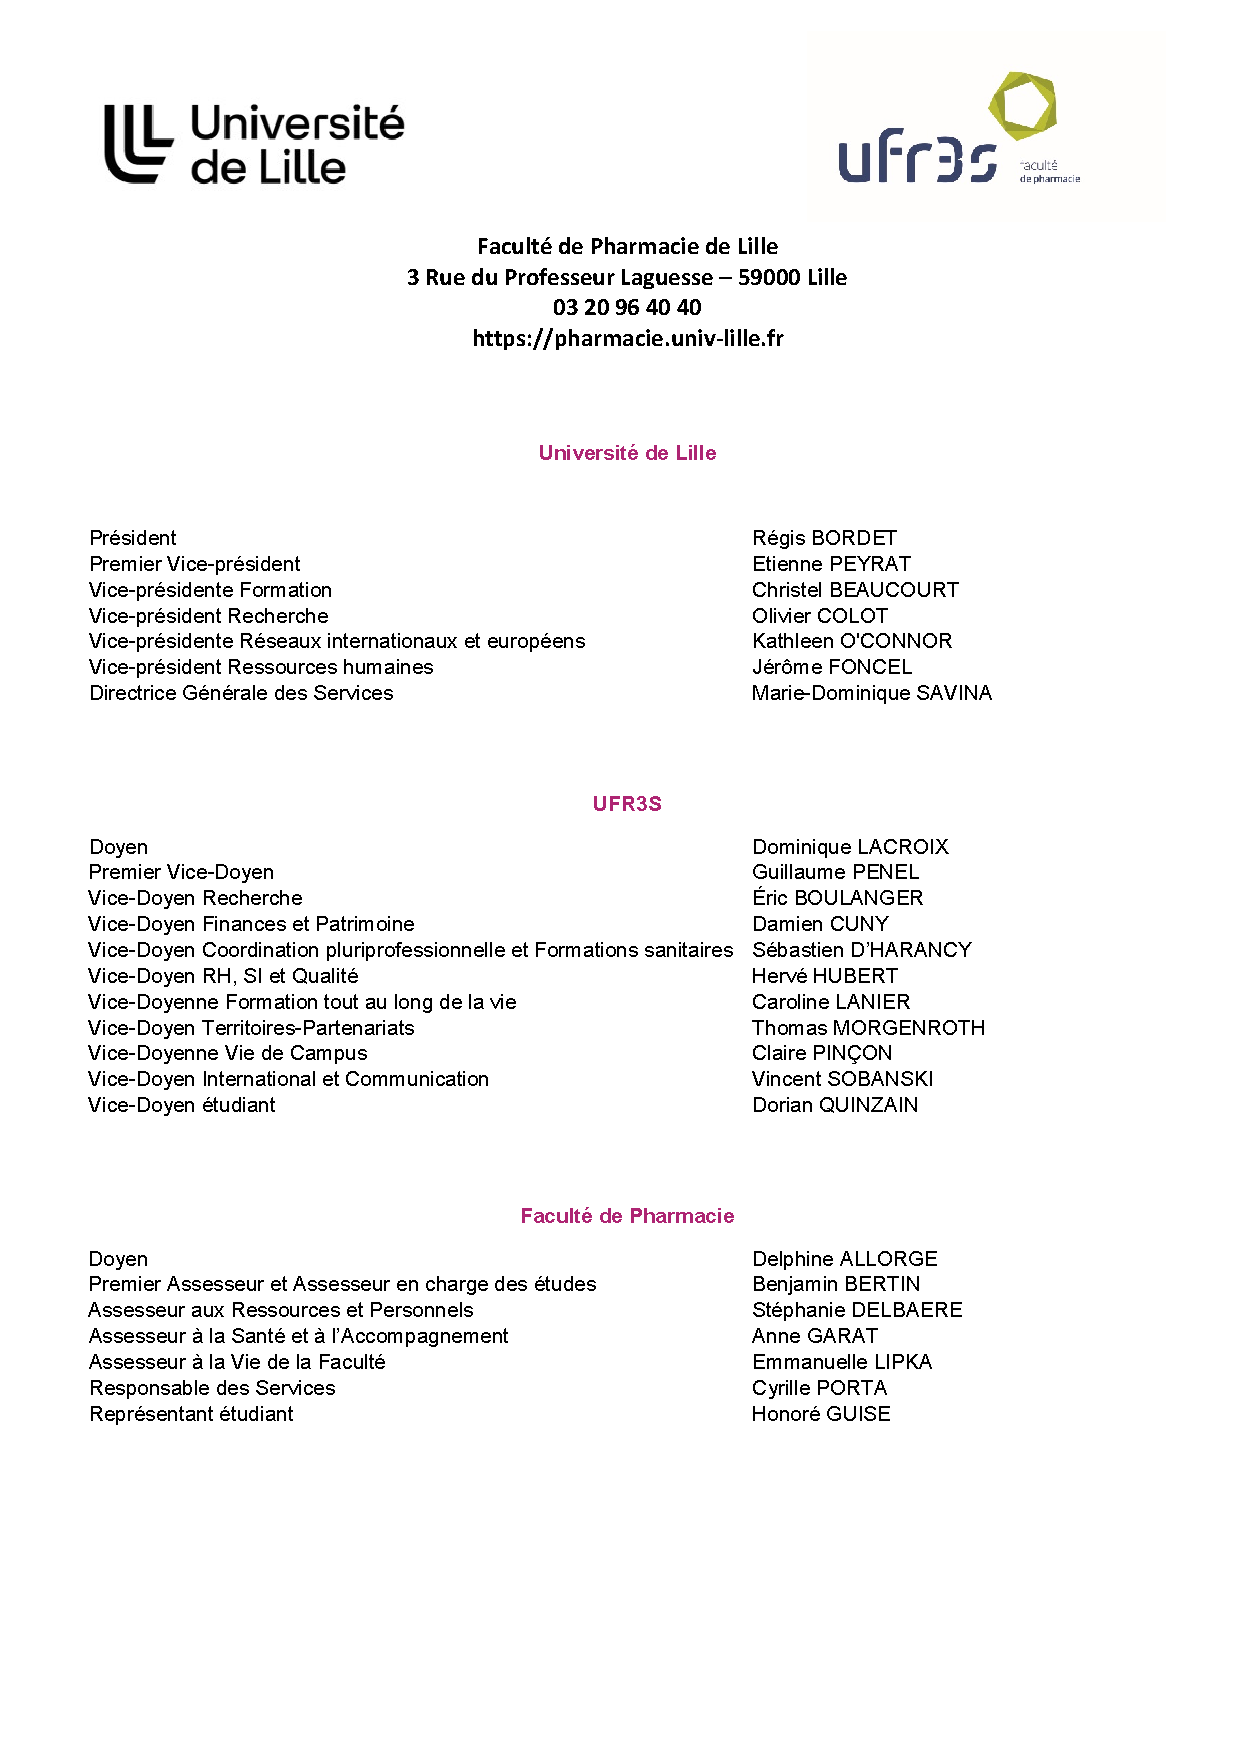
\includepdf[pages={-}]{fac-enseignants2022.pdf} % liste des profs
\cleardoublepage
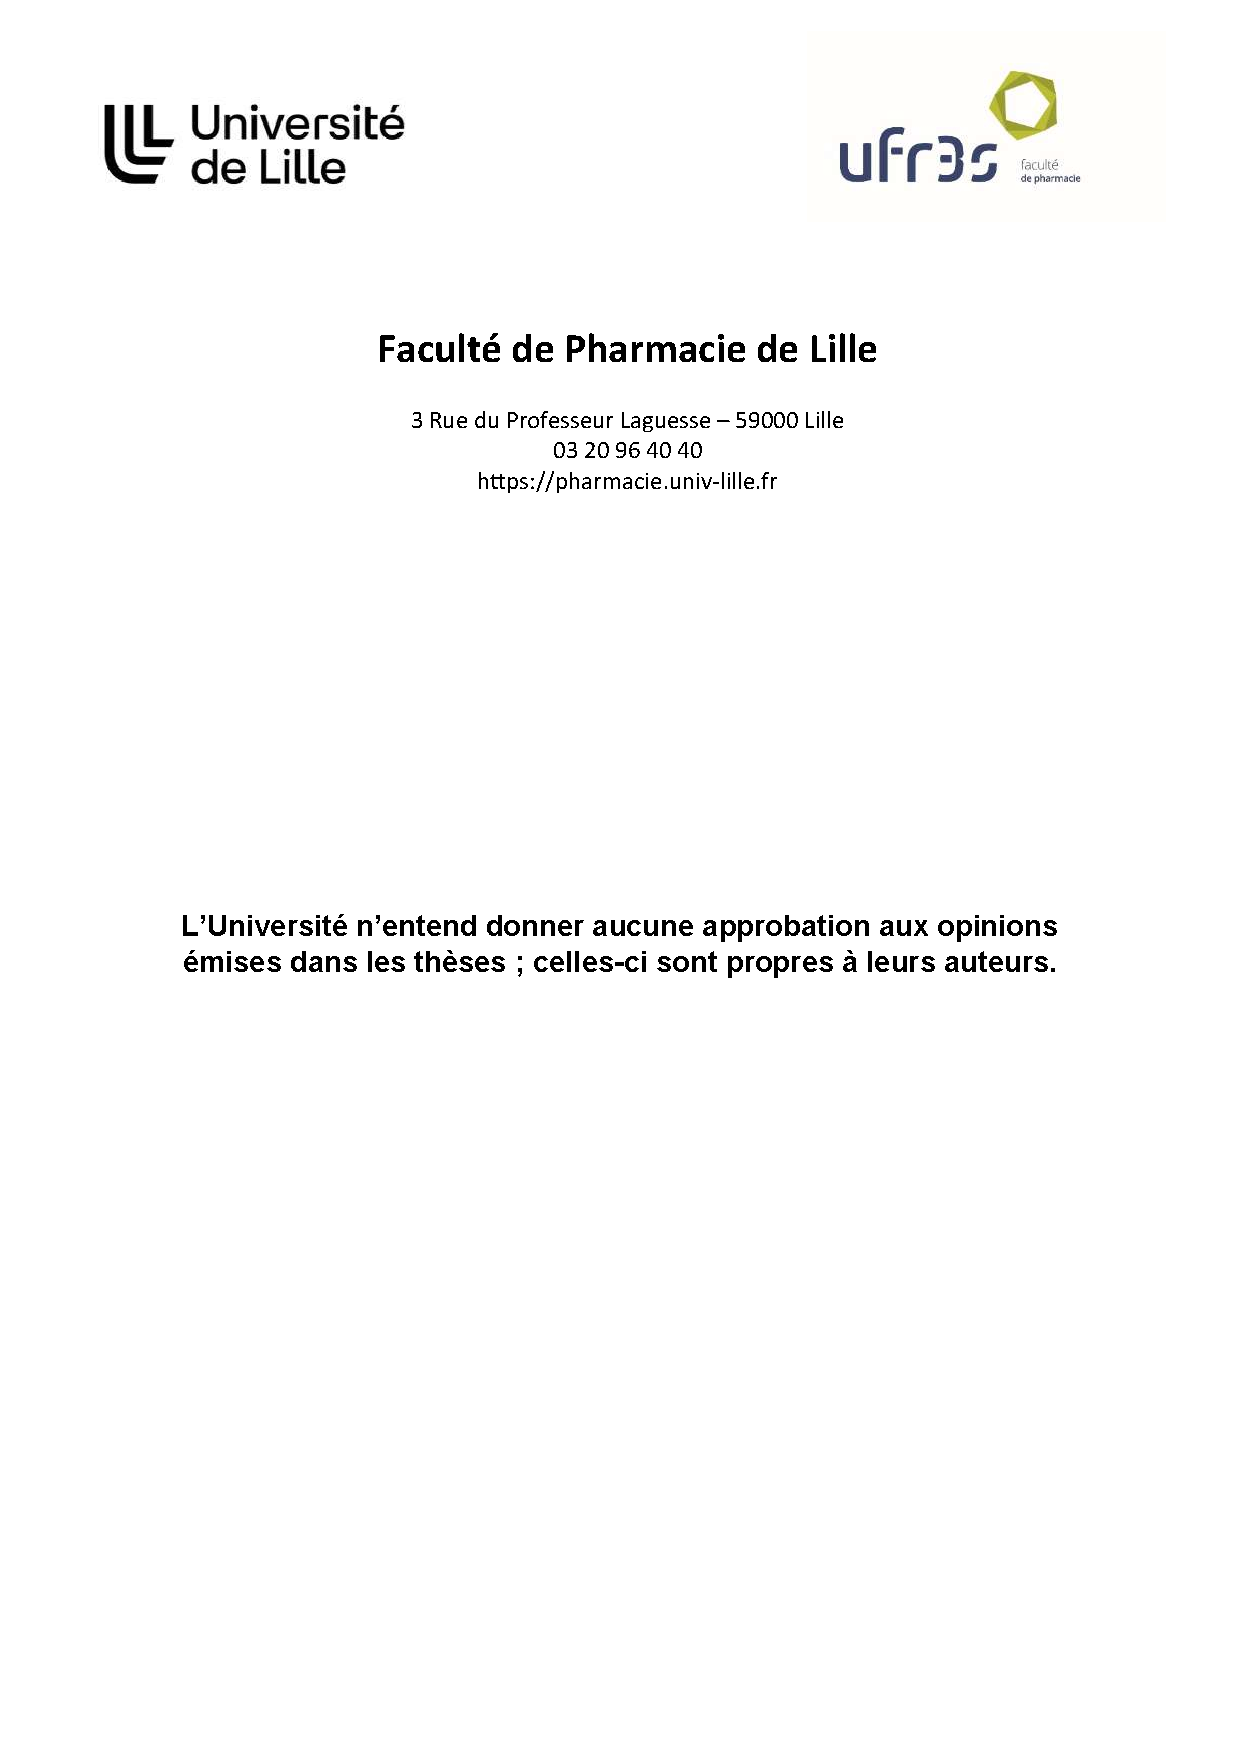
\includepdf[pages={-}]{fac-disclaimer.pdf} % disclaimer opinions
\cleardoublepage
{\rmfamily
~ \\ ~
J'adresse mes sinc\`{e}res remerciements :
\vspace{5mm}
{\itshape 
\paragraph*{}
A Monsieur le Professeur Mohamed \textsc{Lemdani},
\paragraph*{}
Je vous remercie de me faire l'honneur de pr\'{e}sider le jury de ma th\`{e}se, ainsi que pour tous les enseignements que vous avez dispens\'{e}s \`{a} vos \'{e}tudiants depuis la PACES, avec patience et bienveillance. Soyez assur\'{e} de mon profond respect.
\vspace{5mm}
\paragraph*{}
A Monsieur le Docteur Julien \textsc{Hamonier},
\paragraph*{}
Merci pour ta confiance et ton accompagnement dans cette th\`{e}se. Je te remercie pour ton soutien, ta disponibilit\'{e} et tes pr\'{e}cieux conseils dans l'\'{e}laboration et la continuelle am\'{e}lioration de cette th\`{e}se. Sois assur\'{e} de toute ma consid\'{e}ration.
\vspace{5mm}
\paragraph*{}
A Monsieur le Docteur St\'{e}phane \textsc{Welti},
\paragraph*{}
Je te remercie chaleureusement d'avoir accept\'{e} de faire partie de mon jury.  Merci pour tes enseignements qui m'ont fait d\'{e}couvrir toute la diversit\'{e} du monde fongique et la richesse de la mycologie. \\
Merci \'{e}galement pour ton engagement associatif et artistique aux c\^ {o}t\'{e}s des \'{e}tudiants de notre belle facult\'{e}, et pour les tr\`{e}s bons moments pass\'{e}s ensemble.
\vspace{5mm}
\paragraph*{}
A Madame le Docteur Caroline \textsc{Mousset},
\paragraph*{}
Je te suis reconnaissant d'avoir accept\'{e} d'int\'{e}grer le jury de cette th\`{e}se. Merci pour ton accompagnement quotidien et le temps que tu consacres \`{a} ma formation aux missions pharmaceutiques du pharmacien en Assurance Qualit\'{e} op\'{e}rationnelle. \\
Pour le temps et l'\'{e}nergie que tu d\'{e}ploies sans compter, pour ton attention permanente au d\'{e}veloppement de chacun des membres de ton \'{e}quipe, re\c{c}ois l'expression de ma profonde gratitude.
\vspace{5mm}
\paragraph*{}
A Monsieur le Professeur R\'{e}gis \textsc{Courtecuisse},
\paragraph*{}
Pour vos encouragements, votre bienveillance envers vos \'{e}tudiants et -- bien entendu -- pour vos enseignements et ouvrages de r\'{e}f\'{e}rence sans lesquels cette th\`{e}se n'aurait pu voir le jour, je vous remercie infiniment.
\cleardoublepage
\paragraph*{}
A ma famille,
\paragraph*{}
Un grand merci pour votre soutien infaillible, tout particuli\`{e}rement \`{a} mes parents. Votre amour, votre pr\'{e}sence \`{a} mes c\^ {o}t\'{e}s dans les bons moments comme dans les plus difficiles m'ont constamment incit\'{e} \`{a} aller de l'avant, je ne saurais jamais assez vous remercier pour tout ce que vous avez fait pour moi.
\vspace{5mm}
\paragraph*{}
A mes amis de la Facult\'{e} de Pharmacie de Lille,
\paragraph*{}
Merci pour ces moments exceptionnels que j'ai pass\'{e} aupr\`{e}s de vous. Je garde en m\'{e}moire de tr\`{e}s beaux souvenirs et de beaux projets men\'{e}s ensemble. Cette r\'{e}ussite que constitue l'accomplissement de cette th\`{e}se est la n\^ {o}tre, et je suis fier de la partager avec vous.
\paragraph*{}
J'ai eu la chance de passer, au cours de cette derni\`{e}re demi-d\'{e}cennie, des moments inoubliables, que je chérirai toute ma vie. Merci \`{a} Aur\'{e}lie, William, Marion, Cantin, Lucas, Manon, Armand, Marine et Amandine. Un grand merci \'{e}galement \`{a} tous les copains de l'AAEPL (la grande!) et des Zycos.
\vspace{5mm}
\paragraph*{}
A mes confr\`{e}res de l'industrie pharmaceutique,
\paragraph*{}
Merci \`{a} la dream team du Bureau du Bonheur et des Licornes, l'\'{e}quipe d'enfants terribles (et de lib\'{e}rateurs de choc) de Delpharm Lille : Florent, Flavie, Fiora, Gautier, Cem, Hasnein, Samira et Caroline.
\paragraph*{}
Merci pour la belle ambiance, pour la formidable coh\'{e}sion et solidarit\'{e} dont cette \'{e}quipe sait faire preuve, ainsi que pour la saine \'{e}mulation qui nous a pouss\'{e} \`{a} avancer tous ensemble, et \`{a} faire progresser nos projets de th\`{e}se respectifs.
}
}
\cleardoublepage
%\end{document} % POUR TEST
